
%-----------------------------------------------------------------------
%
% filename = usermanual.tex
% 
%-----------------------------------------------------------------------

\documentclass[12pt]{article}

% Load packages for symbols and figures.

\usepackage{latexsym}
\usepackage{epsfig}
\usepackage{amsmath}
\usepackage{amssymb}
\usepackage{tikz}
\usetikzlibrary{shapes}

% Page settings.

\setlength{\textwidth}{170mm}
\setlength{\oddsidemargin}{-5mm}
\setlength{\evensidemargin}{-5mm}


%%%%%%%%%%%%%%%%%%%%%%%%%%
%%%   BEGIN DOCUMENT   %%%
%%%%%%%%%%%%%%%%%%%%%%%%%%

\begin{document}

% Reference equations with section number.

\renewcommand{\theequation}{\thesection.\arabic{equation}}

\parindent 0mm


%%%%%%%%%%%%%%%%%
%%%   TITLE   %%%
%%%%%%%%%%%%%%%%%

\title{Code \texttt{OllinAxis-BiB} \\ User's manual}

\author{Miguel Alcubierre \\
Instituto de Ciencias Nucleares, UNAM \\
malcubi@nucleares.unam.mx}

\date{June, 2022}

\maketitle

\tableofcontents


%%%%%%%%%%%%%%%%%%%%%%%%
%%%   INTRODUCTION   %%%
%%%%%%%%%%%%%%%%%%%%%%%%

\pagebreak

\section{Introduction}

This program solves the Einstein evolution equations in axial symmetry
using a curvilinear version of the BSSN formulation for the 3+1
evolution equations, with different types of matter and different
gauge conditions. \\

The main difference of this version of the code with respect to
previous ones is the fact that it uses box-in-box mesh refinement
(hence the BiB part of the name), and is parallelized with MPI.
Many parts of this code are based on a previous version written
by myself and José Manuel Torres.  An even older version was
written by Milton Ruiz. \\

Note: This manual is TERRIBLY INCOMPLETE!  I haven't had the time to
do it. Still, it should give you a good idea of the basics. I will be
adding a little bit more every now and again. \\


%%%%%%%%%%%%%%%%%%%%
%%%   DOWNLOAD   %%%
%%%%%%%%%%%%%%%%%%%%

\section{Downloading the code}

If you are reading this it means you probably already downloaded the
code.  But if for some reason you need to download it here is how. \\

The easiest way to obtain the code is to download it from GitHub: \\

\texttt{\footnotesize git clone https://github.com/malcubi/OllinAxis-BiB} \\

Once you have the code, you can get updated versions by just doing
``git pull'' inside the code main directory.

\pagebreak


%%%%%%%%%%%%%%%%%%%%%%%
%%%   DIRECTORIES   %%%
%%%%%%%%%%%%%%%%%%%%%%%

\section{Directory structure}

The main directory for the code is \texttt{OllinAxis-BiB}.  There are
several sub-directories inside this main directory:

\begin{list}{}{
\setlength{\leftmargin}{40mm}
\setlength{\labelsep}{10mm}
\setlength{\labelwidth}{25mm}}

\item[\texttt{CVS}] Contains information about the CVS root and server (see
Sec.~\ref{sec:editing}).

\item[\texttt{doc}] Contains the tex and pdf files for this user's
  manual.

\item[\texttt{exe}] This directory is created at compile time and
  contains the executable file.  It also contains a copy of the
  parameter files found in directory \texttt{par} (see below).

\item[\texttt{fakempi}] Contains fake MPI routines so that the
  compiler won't complain if MPI is not installed.

\item[\texttt{gnuplot}] Contains a couple of simple gnuplot macros for
  visualization.

\item[\texttt{objs}] This directory is created at compile time and
  contains all the object and module files.

\item[\texttt{ollingraph}] Contains the visualization packages
  ``ollingraph'' and ``ollingraph2D'' for convenient ``quick and
  dirty'' visualization (see Section~\ref{sec:ollingraph} below).

\item[\texttt{par}] Contains examples of parameter files (see
Section~\ref{sec:parfiles} below).

\item[\texttt{prl}] Contains perl scripts used at compile time to
  create the subroutines that manage parameters and arrays.

\item[\texttt{src}] Contains the source files for all the code
  routines.

\end{list}

\vspace{3mm}

The directory \texttt{src} is itself divided into a series of
sub-directories in order to better classify the different
routines. These sub-directories are:

\begin{list}{}{
\setlength{\leftmargin}{40mm}
\setlength{\labelsep}{10mm}
\setlength{\labelwidth}{25mm}}

\item[\texttt{auto}] Contains \texttt{FORTRAN} files that are
  automatically generated at compile time by the perl scripts.  These
  files should not be edited manually!

\item[\texttt{base}] Contains the routines that control the basic
  execution of the code, including the parameter and array
  declarations, the parameter parser, the output routines, the main
  evolution controllers, and generic routines for calculating
  derivatives, dissipation, etc.  The code in fact starts execution at
  the routine \texttt{main.f90} contained in this directory.

\item[\texttt{elliptic}] Contains routines for solving elliptic
  equations for initial data and/or maximal slicing for example.

\item[\texttt{geometry}] Contains routines related to initial data,
  evolution and analysis of the spacetime geometric variables,
  including sources, gauge conditions, constraints, horizon finders,
  etc.

\item[\texttt{matter}] Contains routines related to the initial data,
  evolution and analysis of the different matter models, including a
  generic routine for calculating the basic matter variables, and
  routines for evolving scalar fields, electric fields, fluids, etc.

\end{list}

\vspace{3mm}


%%%%%%%%%%%%%%%%%%%%%%%%%%%%%%%%%
%%%   COMPILING AND RUNNING   %%%
%%%%%%%%%%%%%%%%%%%%%%%%%%%%%%%%%

The code is written in \texttt{FORTRAN 90} and is parallelized with
\texttt{MPI} (Message Passing Interface).  All subroutines are in
separate files inside the directory \texttt{src} and its
sub-directories.

\subsection{Compiling}
\label{sec:compiling}

To compile just move inside the \texttt{OllinAxis-BiB} directory and
type: \\

\texttt{make} \\

This will first run some perl scripts that create a series of
automatically generated \texttt{FORTRAN} files that will be placed
inside the directory \texttt{src/auto}.  It will then compile all the
\texttt{FORTRAN} routines that it can find inside any of the
sub-directories of \texttt{src} (it will attempt to compile any file
with the extension \texttt{.f90}). \\

The resulting object files and \texttt{FORTRAN} module files will be
placed inside the sub-directory \texttt{objs}. The Makefile will then
create a directory \texttt{exe} and will place in it the final
executable file called \texttt{ollinaxis}.  It will also copy to this
directory all the sample parameter files inside the sub-directory
\texttt{par}, and the visualization package \texttt{ollingraph}. \\

Notice that at this time the Makefile can use the compilers
\texttt{g95}, \texttt{gfortran}, or the Intel compilers \texttt{ifc}
and \texttt{ifort}, and it will automatically check if they are
installed. If you have a different compiler then the Makefile will
have to be modified (hopefully it won't be very difficult). The code
will also attempt to find an \texttt{MPI} installation (it looks for
the command \texttt{mpif90}), and if it does not find it it will use
the fake routines inside the directory \texttt{fakempi}. \\

The Makefile has several other useful targets that can be listed by
typing: \texttt{make help}. \\


\subsection{Running}
\label{sec:running}

To run the code move into the directory \texttt{exe} and type: \\

\texttt{ollinaxis name.par} \\

Where \texttt{name.par} is the name of your parameter file (more on
parameter files below).  The code will then read data from the
parameter file silently and hopefully start producing some output to
the screen. The code will also create an output directory and will
write the data files to that directory. \\

For parallel runs using \texttt{MPI} one must use instead the command:
\\

\texttt{mpirun -np N ollinaxis name.par} \\

where \texttt{N} should be an integer number that specifies the number
of processors to be used. \\


%%%%%%%%%%%%%%%%%%%%%%%%%%%
%%%   PARAMETER FILES   %%%
%%%%%%%%%%%%%%%%%%%%%%%%%%%

\section{Parameter files}
\label{sec:parfiles}

At run time the code reads the parameter values from a parameter file
(parfile), with a name of the form \texttt{name.par}, that must be
specified in the command line after the executable: \\

\texttt{ollinaxis  name.par} \\

The data in this parameter file can be given in any order, using the
format: \\

\texttt{parameter = value} \\

Comments (anything after a \texttt{\#}) and blank lines are ignored.
Only one parameter is allowed per line, and only one value is allowed
per parameter, with the exception of the parameters
\texttt{outvars0D}, \texttt{outvars1D} and \texttt{outvars2D} that
control which arrays get output and take lists of arrays as values,
for example: \\

\texttt{outvars0D = alpha,A,B,C,H} \\

There is in fact one other parameter that can also take multiple
values as input, it is the parameter \texttt{mattertype} that can
accept several types of matter at once (see Section~\ref{sec:matter}
below).\\

Parameters that do not appear in the parfile get the default values
given in the file \texttt{src/base/param.f90}.  Examples of parameter
files can be found in the subdirectory \texttt{par}. \\

IMPORTANT: Even though \texttt{FORTRAN} does not distinguish between
upper and lower case in variable names, the names of parameters are
handled as strings by the parameter parser, so lower and upper case
are in fact different.  The name of parameters in the parameter file
should then be identical to the way in which they appear in the file
\texttt{param.f90}. \\


%%%%%%%%%%%%%%%%%%%%%%%%
%%%   OUTPUT FILES   %%%
%%%%%%%%%%%%%%%%%%%%%%%%

\section{Output files}

At run time, the codes creates an output directory whose name should
be given in the parameter file. It then produces a series of output
files with the data from the run. There are so called \texttt{0D}
files (with extension \texttt{*.tl}), \texttt{1D} files (with
extensions \texttt{*.rl}, \texttt{*.zl} and \texttt{*.dl}), and
\texttt{2D} files (with extension \texttt{*.2D}). \\

The \texttt{OD} files refer to scalar quantities obtained from the
spatial arrays as functions of time. These scalar quantities include
the maximum (\texttt{max}), the minimum (\texttt{min}), and three
different norms of the spatial arrays: maximum absolute value
(\texttt{nm1}), root mean square (\texttt{nm2}), and total variation
(\texttt{var}). The value of different variables at the origin is also
output. \\

The \texttt{1D} files contain the complete arrays along the coordinate
axis and diagonals at different times, while the \texttt{2D} files
output the full arrays.  Beware: If you do output very often these
files can become quite large! \\

Since we can have several grid refinement levels, and grid boxes,
the file names are appended with a number corresponding to the specific
box and level (all grid levels have output). For example: \\

\texttt{alphab0l0.rl}: \hspace{5mm} Level 0 (coarsest grid) \\
\texttt{alphab0l1.rl}: \hspace{5mm} Level 1 \\
... \\

All files are written in ASCII, and using a format adapted to XGRAPH
(but other graphic packages should be able to read them).\\

Output is controlled by the following parameters:

\begin{list}{}{
\setlength{\leftmargin}{35mm}
\setlength{\labelsep}{10mm}
\setlength{\labelwidth}{20mm}}

\item[\texttt{directory}] Name of directory for output.

\item[\texttt{Ninfo}] How often do we output information to screen?

\item[\texttt{Noutput0D}] How often do we do 0D output?

\item[\texttt{Noutput1D}] How often do we do 1D output?

\item[\texttt{Noutput2D}] How often do we do 2D output?

\item[\texttt{outvars0D}] Arrays that need 0D output (a list separated by commas).

\item[\texttt{outvars1D}] Arrays that need 1D output (a list separated by commas).

\item[\texttt{outvars2D}] Arrays that need 2D output (a list separated by commas).

\end{list}

\vspace{3mm}


%%%%%%%%%%%%%%%%%%%%%%
%%%   CHECKPOINT   %%%
%%%%%%%%%%%%%%%%%%%%%%


%%%%%%%%%%%%%%%%
%%%   GRID   %%%
%%%%%%%%%%%%%%%%

\setcounter{equation}{0}
\section{Numerical grid}
\label{sec:grid}

\subsection{Grid structure and staggering of the axis}

The code works in cylindrical coordinates $(r,z)$, where $r$
represents distance to the axis of symmetry (not distance to the
origin!), and $z$ the height above or below the ``equator''.  Grid
functions are represented by $f_(i,j)$, with the index $i$
representing the $r$ position, and the index $j$ the $z$ position. \\

In order to avoid having divisions by zero in some terms, we stagger
the symmetry axis. This means that there is no grid point at $r=0$.
Instead, the first grid point (grid point 0) is located at $r=-dr/2$
(with $dr$ the grid spacing), the second one (grid point 1) at
$r=+dr/2$, and so on. This also makes it easy to apply symmetry
boundary conditions, since for an even grid function $f_{(i,j)}$ we
can simply take $f_{0,j}=+f_{1,j}$, and for an odd function
$f_{0,j}=-f_{1,j}$. \\

Grid points to the left of symmetry axis are known as ``ghost
points'', and the code usually adds more than one in order to be able
to use higher order differencing stencils. The positions of the grid
points along the $r$ direction then correspond to $r_i = (i-1/2)*dr$,
where $i$ runs from $(1-g)$ to some maximum number \texttt{Nr}, and
where $g$ is the number of ghost points given by the parameter
\texttt{ghost}.  In fact, for second order spatial differencing the
code takes \texttt{ghost=2}, while for fourth order differencing it
takes \texttt{ghost=3}, see Figure~\ref{fig:grid} (the reason for this
has to do with dissipation, which typically needs one extra ghost
point that would normally be required for a given differencing order,
see below). Notice that the parameter \texttt{ghost} is determined by
the code at run time and should NOT be fixed in the parameter file. \\

\begin{figure}[t]
\begin{center}
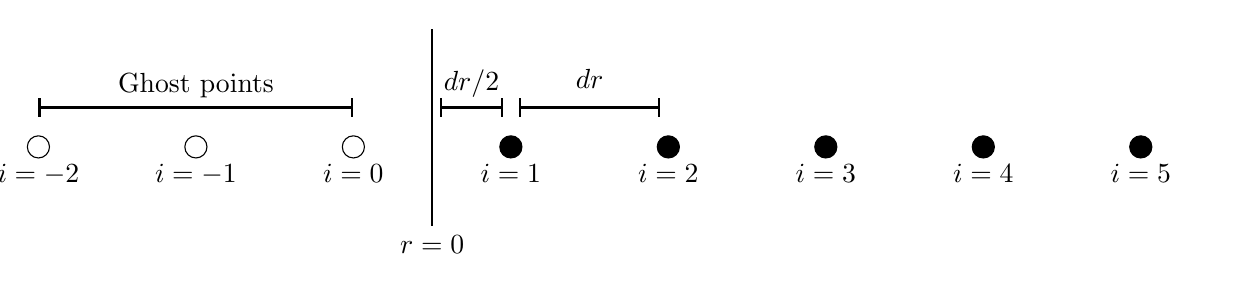
\begin{tikzpicture}
\draw[black] (-3,0) circle (4pt);
\node [below] at (-3,-0.1) {$i=-2$};
\draw[black] (-1,0) circle (4pt);
\node [below] at (-1,-0.1) {$i=-1$};
\draw[black] (1,0) circle (4pt);
\node [below] at (1,-0.1) {$i=0$};
\filldraw[black] (3,0) circle (4pt);
\node [below] at (3,-0.1) {$i=1$};
\filldraw[black] (5,0) circle (4pt);
\node [below] at (5,-0.1) {$i=2$};
\filldraw[black] (7,0) circle (4pt);
\node [below] at (7,-0.1) {$i=3$};
\filldraw[black] (9,0) circle (4pt);
\node [below] at (9,-0.1) {$i=4$};
\filldraw[black] (11,0) circle (4pt);
\node [below] at (11,-0.1) {$i=5$};
\draw[black,thick,|-|] (2.1,0.5) -- (2.9,0.5);
\node[above] at (2.5,0.5) {$dr/2$};
\draw[black,thick,|-|] (3.1,0.5) -- (4.9,0.5);
\node[above] at (4,0.62) {$dr$};
\draw[black,thick] (2,-1) -- (2,1.5);
\node [below] at (2,-1) {$r=0$};
\draw[black,thick,|-|] (-3,0.5) -- (1,0.5);
\node [above] at (-1,0.5) {Ghost points};
\end{tikzpicture}
\end{center}
\caption{Basic grid structure close to the axis of symmetry $r=0$,
  showing how the axis is staggered.  We show the case of 3 ghost
  points to the left of the origin (for fourth order spatial
  differencing).}
\label{fig:grid}
\end{figure}

The grid for the coordinate $z$, on the other hand, has two different
structures depending on whether we have or not equatorial symmetry.
If the logical parameter \texttt{eqsym} is set to \texttt{.false.}, 
that is if there is no equatorial symmetry, then the grid uses \texttt{Nz}
points along the $z$ direction starting from $-Nz/2$ to $+Nz/2$.  Notice
that of \texttt{Nz} is even then there will be no point at $z=0$ (and the
equator will be staggered9, while if \texttt{Nz} is odd there will be
a point with $z=0$.

On the other hand, if the logical parameter \texttt{eqsym} is set to
\texttt{.true.}, then the equator is always staggered and symmetry
conditions are applied in the $z$ direction in the same way as it is
done with the axis if symmetry for the coordinate $r$. Having
equatorial symmetry then reduces the use of computational by half.

\subsection{Box-in-box grid refinement}

The also code uses ``box-in-box'' type grid refinement.  That is, it
has refinement levels with higher resolution ...


%%%%%%%%%%%%%%%%%%%%%
%%%   SPACETIME   %%%
%%%%%%%%%%%%%%%%%%%%%

\setcounter{equation}{0}
\section{Spacetime and evolution equations}

\subsection{Spacetime metric}

As already mentioned, the code uses cylindrical coordinates $(r,z)$ in
space. Notice that what the code calls $r$ here represents distance to
the symmetry axis and not distance to the origin. The distance to the
origin in the code is in fact called $rr:=(r^2 + z^2)^{1/2}$. \\

The spatial metric is written in the following way:
\begin{align}
dl^2 &= e^{4 \phi(r,z,t)} \left[ A(r,z,t) dr^2 + B(r,z,t) dz^2 
+ r^2 H(r,z,t) d\varphi^2 \right. \nonumber \\
&+ 2 \left. r \left( C(r,z,t) dr dz + r^2 C_1(r,z,t) dr d\varphi
+ r C_2(r,z,t) dz d\varphi \right) \right] \; ,
\label{eq:metric}
\end{align}
with $\phi$ the conformal factor. The powers of $r$ in some of the
terms come from the behaviour of the different metric components close
to the axis. Factorizong those powers of $r$ exoplicitely allows us to
make sure that the functions $(A,B,H,C,C_1,C_2)$ are well behaved at
$r=0$. Notice that the components of the extrinsic curvature $K_{ij}$
are also decomposed in a similar way (see below). \\

We also define the function $\psi = e^\phi$ and use it instead of
$\phi$ in many expressions. For the lapse function we use the array
$\alpha(r,z,t)$, while the shift in principle has three components:
$\beta^r(r,z,t)$, $\beta^z(r,z,t)$, $\beta^\varphi(r,z,t)$. \\

Notice that when there is no angular momentum the metric can be
simplified since in that case we have $\beta^\varphi=0$, and
$C_1=C_2=0$.  The code controls this using the logical parameter
\texttt{angmom}: if this parameter is true then those arrays are
turned on, while if it is false they are off.  By default the
parameter is false, so that those arrays are turned off. \\

It is also useful to define an inverse to the conformal factor as:
\begin{equation}
\chi := 1/\psi^n = \exp(-n \phi) \; ,
\end{equation}
with $n$ a power controlled by the parameter \texttt{chipower}.  For
black hole spacetimes the conformal factor $\phi$ is singular at the
black hole position, while $\chi$ remains regular, so it is best
to evolve $\chi$ instead of $\phi$. This can be controlled with the
logical parameter \texttt{chimethod} (which by default is set to
\texttt{.true.}).

\subsection{Evolution equations}

For the evolution equations, the code uses a
Baumgarte-Shapiro-Shibata-Nakamura (BSSN) formulation adapted to axial
symmetry.  The specific form of the evolution equations used here can
be found in~\cite{Alcubierre11}. \\

There are two BSSN variants or ``flavors'' controlled by the
parameter \texttt{bssnflavor}, which can take the values
\texttt{lagrangian} or \texttt{eulerian} (the
default is \texttt{bssnflavor=lagrangian}). They refer to the way in which the
shift terms are added to make determinant of the conformal metric
constant along time-lines (lagrangian), or constant along the
normal-lines (eulerian). \\

There is also a parameter that allows one to switch off the evolution
of the spacetime, which is useful in case one wants to evolve some
matter field in a fixed background spacetime. The parameter is called
\texttt{spacetime} and can have the values \texttt{dynamic} or
  \texttt{static} (default is \texttt{spacetime=dynamic}). \\

The main evolution variables (arrays) are:

\begin{list}{}{
\setlength{\leftmargin}{35mm}
\setlength{\labelsep}{10mm}
\setlength{\labelwidth}{20mm}}

\item[\texttt{alpha}] The lapse function $\alpha$.

\item[\texttt{beta\_r}] Contravariant shift component $\beta^r$.

\item[\texttt{beta\_z}] Contravariant shift component $\beta^z$.

\item[\texttt{beta\_p}] Contravariant angular shift component $\beta^\varphi$.

\item[\texttt{phi}] The conformal factor $\phi$ (see equation~\ref{eq:metric}).

\item[\texttt{psi}] The conformal factor $\psi=e^\phi$ (see
  equation~\ref{eq:metric}).

\item[\texttt{A}] Component $(r,r)$ of conformal metric $\tilde{g}_{rr}=\texttt{A}$.

\item[\texttt{B}] Component $(z,z)$ of conformal metric  $\tilde{g}_{zz}=\texttt{B}$.

\item[\texttt{H}] Component $(\varphi,\varphi)$ of conformal metric  $\tilde{g}_{\varphi \varphi}= r^2 \: \texttt{H}$.

\item[\texttt{C}] Component $(r,z)$ of conformal metric  $\tilde{g}_{rz}= r \: \texttt{C}$.

\item[\texttt{C1}] Component $(r,\varphi)$ of conformal metric $\tilde{g}_{r \varphi}= r^2 \: \texttt{C1}$.

\item[\texttt{C2}] Component $(z,\varphi)$ of conformal metric $\tilde{g}_{z \varphi}= r \: \texttt{C1}$.

\item[\texttt{trK}] Trace of the extrinsic curvature
  \mbox{$\texttt{trK} := {K^m}_m$}.

\item[\texttt{KTA}] Component $(r,r)$ of conformal trace-free extrinsic
  curvature $\tilde{K}^{TF}_{rr} = \texttt{KTA}$.

\item[\texttt{KTB}] Component $(z,z)$ of conformal trace-free extrinsic
  curvature $\tilde{K}^{TF}_{rr} = \texttt{KTA}$.

\item[\texttt{KTH}] Component $(\varphi,\varphi)$ of conformal trace-free extrinsic
  curvature $\tilde{K}^{TF}_{\varphi \varphi} = r^2 \: \texttt{KTH}$.

\item[\texttt{KTC}] Component $(r,z)$ of conformal trace-free extrinsic
  curvature $\tilde{K}^{TF}_{rz} = r \: \texttt{KTC}$.

\item[\texttt{KTC1}] Component $(r,\varphi)$ of conformal trace-free extrinsic
  curvature $\tilde{K}^{TF}_{r \varphi} = r^2 \: \texttt{KTC1}$.

\item[\texttt{KTC2}] Component $(r,\varphi)$ of conformal trace-free extrinsic
  curvature $\tilde{K}^{TF}_{z \varphi} = r \: \texttt{KTC2}$.

\item[\texttt{Delta\_r}] Contravariant component of auxilary BSSN variable $\Delta^r$.

\item[\texttt{Delta\_z}] Contravariant component of auxilary BSSN variable $\Delta^z$.

\item[\texttt{Delta\_p}] Contravariant component of auxilary BSSN variable $\Delta^\varphi$.

\end{list}

Notice that, even though the auxiliary BSSN variables $\Delta^i$ are
initially defined in terms of metric derivatives, they are later
evolved independently with their own evolution equations (modified using
the momentum constraints), as required in the BSSN formulation. \\

The code also calculates a series of auxiliary geometric quantities
defined as:

\begin{list}{}{
\setlength{\leftmargin}{35mm}
\setlength{\labelsep}{10mm}
\setlength{\labelwidth}{20mm}}

\item[\texttt{psi}] The conformal factor $\texttt{psi}:=\psi=e^\phi$.
  The code also calculates $\texttt{psi2}:=\psi^2$ and
    $\texttt{psi4}:=\psi^4$.

\item[\texttt{chi}] Another form of the conformal factor
  $\texttt{chi}=\chi=1/\psi^n$.  This function is in fact evolved
  instead of $\phi$ if one sets the logical parameter
  \texttt{chimethod=.true.} (by default it is true).  This is useful
  for black hole evolutions as it improves the treatment of the
  central punctures.

\end{list}


%%%%%%%%%%%%%%%%%%%%%%%%%%
%%%   REGULARIZATION   %%%
%%%%%%%%%%%%%%%%%%%%%%%%%%


%%%%%%%%%%%%%%%%%%
%%%   MATTER   %%%
%%%%%%%%%%%%%%%%%%

\setcounter{equation}{0}
\section{Matter}
\label{sec:matter}


%%%%%%%%%%%%%%%%%%%%%%%
%%%   CONSTRAINTS   %%%
%%%%%%%%%%%%%%%%%%%%%%%


%%%%%%%%%%%%%%%%%%%%%%%%%%%%%%
%%%   SLICING CONDITIONS   %%%
%%%%%%%%%%%%%%%%%%%%%%%%%%%%%%

\setcounter{equation}{0}
\section{Slicing conditions}
\label{sec:slicing}


%%%%%%%%%%%%%%%%%%%%%%%%%%%%
%%%   SHIFT CONDITIONS   %%%
%%%%%%%%%%%%%%%%%%%%%%%%%%%%

\setcounter{equation}{0}
\section{Shift conditions}
\label{sec:shift}


%%%%%%%%%%%%%%%%%%%%%%%%%%%%%%%
%%%   BOUNDARY CONDITIONS   %%%
%%%%%%%%%%%%%%%%%%%%%%%%%%%%%%%


%%%%%%%%%%%%%%%%%%%%%%%%
%%%   INITIAL DATA   %%%
%%%%%%%%%%%%%%%%%%%%%%%%

\setcounter{equation}{0}
\section{Initial data}
\label{sec:initial}

The type of initial data is controlled by the character-type parameter
\texttt{idata}.  If you add a new type of initial data it should be
appended to the list of allowed values for this parameter in the file
\texttt{src/base/param.f90}.  You should also add a corresponding call to your
initial data routine in the file \texttt{src/base/initial.f90}. \\


%%%%%%%%%%%%%%%%%%%%
%%%   HORIZONS   %%%
%%%%%%%%%%%%%%%%%%%%


%%%%%%%%%%%%%%%%%%%%%%%%%%%%%
%%%   NUMERICAL METHODS   %%%
%%%%%%%%%%%%%%%%%%%%%%%%%%%%%

\setcounter{equation}{0}
\section{Numerical methods}
\label{sec:numerics}

\subsection{Time integration}

For the time integration the code uses a method of lines, where the
time integration and spatial differentiation are considered
independent of each other. \\


%%%%%%%%%%%%%%%%%%%%%%%%%%%%
%%%   ELLIPTIC SOLVERS   %%%
%%%%%%%%%%%%%%%%%%%%%%%%%%%%


%%%%%%%%%%%%%%%%%%%%%%%%%%%%%%
%%%   LIST OF PARAMETERS   %%%
%%%%%%%%%%%%%%%%%%%%%%%%%%%%%%

\section{List of main code parameters}
\label{sec:parameters}


%%%%%%%%%%%%%%%%%%%%%%%%%%%%
%%%   EDITING THE CODE   %%%
%%%%%%%%%%%%%%%%%%%%%%%%%%%%

\section{Editing the code}
\label{sec:editing}


%%%%%%%%%%%%%%%%%%%%%%
%%%   OLLINGRAPH   %%%
%%%%%%%%%%%%%%%%%%%%%%

\section{Ollingraph}
\label{sec:ollingraph}

The code includes a simple 1D visualization package called
``ollingraph''.  It is written in Python and uses Matplotlib to plot
simple line plots and animations.  At the moment it should work fine
under python 3.11. It is supposed to have similar functionality to
the old xgraph and ygraph packages, and expects the data files in the
same format (see below). \\

The plots are quite simple, and meant for quick/dirty interactive
visualization.  These plots are not supposed to be used for figures
intended for publication (use gnuplot or something similar for
that). To use the package type: \\

\texttt{ollingraph  file1 file2 ... filen} \\

When plotting several data files at once, they are all assumed to be
of the same type.  One can also add a custom name for the plot using
the option --title: \\

\texttt{ollingraph --title="Plot name" file1 file2 ... filen} \\

If this option is not there the plot is just named after the name of
the data file being plotted, assuming there is only one, or just says
``Multiple data files'' if there is more than one file. \\

Before using it make sure that \texttt{ollingraph} has execution
permission: \\

\texttt{chmod +x ollingraph} \\

There is also a package for simple plots of 2D arrays called
\texttt{ollingraph2D}. It is called in a similar way:

\texttt{ollingraph2D  file} \\

But in this case the file to be plotted must have extension
\texttt{.2D}.

\vspace{5mm}

The data files are expected to have the following format:

\begin{itemize}

\item 0D files (those ending in .tl):

\begin{enumerate}

\item One comment line starting with \texttt{\#} or \texttt{"} with
  the file name (this line could be missing and it should still work).

\item A series of lines with the data points, with the x and y values
  separated by blank spaces.

\end{enumerate}

\item 1D evolution-type files (those ending in .rl):

\begin{enumerate}

\item Each time step begins with a comment line starting with
  \texttt{\#} or \texttt{"} that contains the time in the format: \\

\texttt{\#Time = (real number)} \\

\item A series of lines with the data points, with the x and y values
  separated by blank spaces.

\item One or more blank lines to separate the next time step.

\end{enumerate}

\end{itemize}


%%%%%%%%%%%%%%%%%%%%%%
%%%   REFERENCES   %%%
%%%%%%%%%%%%%%%%%%%%%%

\begin{thebibliography}{99}

\bibitem{Alcubierre08} ``Regularization of spherical and axisymmetric
  evolution codes in numerical relativity'', M. Ruiz, M. Alcubierre,
  D. Nuñez, Gen.Rel.Grav. {\bf 40}, 159-182 (2008); arXiv:0706.0923
  [gr-qc].

\bibitem{Alcubierre11} ``Formulations of the 3+1 evolution equations
  in curvilinear coordinates'', M.~Alcubierre and M.~D.~Mendez,
  Gen.Rel.Grav. {\bf 43}, 2769 (2011); arXiv:1010.4013 [gr-qc].

\end{thebibliography}


%%%%%%%%%%%%%%%
%%%   END   %%%
%%%%%%%%%%%%%%%

\end{document}

